\documentclass[11pt]{article}
\usepackage[margin=1in]{geometry}

\usepackage[expansion=false]{microtype}
\usepackage{amsmath,amssymb}
\usepackage{booktabs,tabularx,array}
\usepackage{enumitem}
\usepackage{xcolor}
\usepackage{tikz}
\usetikzlibrary{positioning,arrows.meta,fit,calc}
\usepackage[hidelinks]{hyperref}

\setlist{itemsep=2pt,topsep=3pt}
\newcolumntype{L}{>{\raggedright\arraybackslash}X}
\newcolumntype{P}[1]{>{\raggedright\arraybackslash}p{#1}}
% Claims not yet checked against the primary source.
\newcommand{\verify}{\textsuperscript{\textcolor{red!70!black}{[verify]}}}
\newcommand{\todo}[1]{\textcolor{blue!60!black}{[TODO: #1]}}

\title{A measurement-based study of in-orbit inference\\[2pt]
\large Working notes: setup, facets, and evidence base}
\author{P.\ (Columbia)}
\date{October 6, 2026}

\begin{document}
\maketitle

\section{Thesis and shape of the study}

In-orbit inference is a fixed-rate producer feeding a scarce, intermittent consumer under an energy budget
that changes around the orbit. The producer is the sensor: an imager emitting a frame every 1--30\,s, or
an RF front end streaming IQ samples at a hard rate. The consumer is the downlink, open only during
ground contacts of a few minutes each, a handful of times per day per station. The input channel is stale
in a different way than in robotics: reference imagery, models, and tasking are uplinked from the ground
and can be hours to days old by the time they are used. Published systems work (Kodan, Earth+, Serval,
EarthSight) treats onboard compute as a fixed throughput number; commercial operators (Kepler, Loft)
have deployed Jetson Orins in orbit but, by Loft's own account, there are no public performance
benchmarks.

The hypothesis to test is the same as for physical AI: \textbf{in-orbit inference fails at the interfaces
between layers, not inside the model.} Workload$\leftrightarrow$model is cadence and staleness;
non-model load$\leftrightarrow$model is contention; model$\leftrightarrow$device is energy, thermal,
and transport. Orbit adds one interface robotics does not have: device$\leftrightarrow$environment,
i.e.\ radiation-induced faults. If the hypothesis holds, the fix is a runtime (scheduling, isolation,
energy-aware admission), not a smaller model.

The study is a measurement grid. Each cell is a configuration of the stack below; each cell yields a
failure classification and a task-quality number.

\subsection{The stack}

\begin{center}
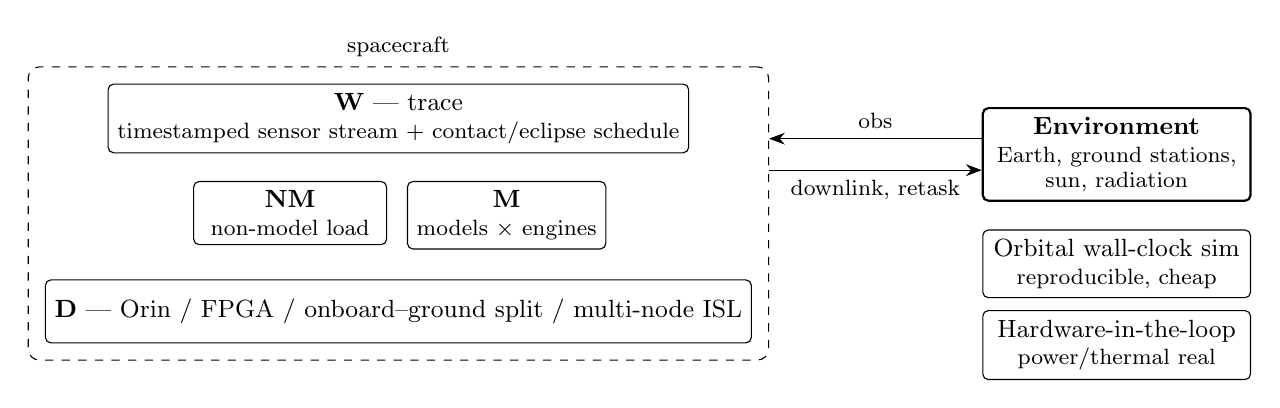
\begin{tikzpicture}[
  box/.style={draw, rounded corners=2pt, minimum width=5.2cm, minimum height=0.8cm, align=center, font=\small},
  side/.style={draw, rounded corners=2pt, minimum width=3.4cm, minimum height=0.8cm, align=center, font=\small},
  world/.style={draw, thick, rounded corners=2pt, minimum width=3.4cm, minimum height=1.0cm, align=center, font=\small},
  >={Stealth[length=2mm]}]
  \node[box] (W) {\textbf{W} --- trace\\[-1pt]\footnotesize timestamped sensor stream + contact/eclipse schedule};
  \node[box, below=0.35cm of W, minimum width=2.45cm, xshift=-1.375cm] (NM) {\textbf{NM}\\[-1pt]\footnotesize non-model load};
  \node[box, below=0.35cm of W, minimum width=2.45cm, xshift=1.375cm] (M) {\textbf{M}\\[-1pt]\footnotesize models $\times$ engines};
  \node[box, below=1.6cm of W] (D) {\textbf{D} --- Orin / FPGA / onboard--ground split / multi-node ISL};
  \node[draw, dashed, rounded corners=4pt, inner sep=6pt, fit=(W)(NM)(M)(D), label={[font=\footnotesize]above:spacecraft}] (sc) {};
  \node[world, right=2.7cm of sc.east, yshift=0.75cm] (E) {\textbf{Environment}\\[-1pt]\footnotesize Earth, ground stations,\\[-2pt]\footnotesize sun, radiation};
  \draw[->] ($(E.west)+(0,0.2)$) -- node[above, font=\footnotesize]{obs} ($(sc.east |- E.west)+(0,0.2)$);
  \draw[<-] ($(E.west)+(0,-0.2)$) -- node[below, font=\footnotesize]{downlink, retask} ($(sc.east |- E.west)+(0,-0.2)$);
  \node[side, below=0.35cm of E] (sim) {Orbital wall-clock sim\\[-1pt]\footnotesize reproducible, cheap};
  \node[side, below=0.15cm of sim] (hil) {Hardware-in-the-loop\\[-1pt]\footnotesize power/thermal real};
\end{tikzpicture}
\end{center}

W, NM, M, and D are all on the spacecraft. The environment is the only source of observations and the
only consumer of output: ground stations receive the downlink, and a retasking decision changes what the
sensor sees next. As in the physical AI notes, W is a recording of what the environment emitted, and the
sim sits beside D as the environment's counterpart, not above W.

\subsection{Execution modes and what each can measure}

\begin{center}
\small
\begin{tabularx}{\textwidth}{@{}P{2.6cm}LL@{}}
\toprule
\textbf{Mode} & \textbf{Mechanism} & \textbf{Measures} \\
\midrule
Trace replay & Stored W (frames sequenced along a propagated ground track) fed to M as fast as the
cadence allows; outputs logged, environment off. Open-loop. &
Throughput vs.\ cadence, contention, energy per frame. Latency distribution of M under NM and D.
Reproducible. \\
\addlinespace
Orbital wall-clock sim & Orbit propagator (SGP4) drives sensor cadence, contact windows, and
sunlight/eclipse power in real time during passes; idle gaps compressed. M runs on the real device in a
separate process. Backlog and storage evolve across passes. &
Cadence misses, backlog/storage overflow, capture-to-alert latency, retask success. The only mode in
which a late decision changes the next observation. \\
\addlinespace
Hardware-in-the-loop & Same loop with the device power-capped to an orbit-average budget, in a
fan-less enclosure (conduction-only proxy), with fault injection. &
Thermal throttling, sustained-vs-burst behavior, energy budget violations, fault tolerance.
Validates that the sim's power/thermal model is not lying. \\
\addlinespace
Real orbit (optional) & Rented compute on a commercial bus (Loft virtual mission, Kepler). &
Ground truth. Expensive, slow, not reproducible; useful as a single anchoring point. \\
\bottomrule
\end{tabularx}
\end{center}

Why wall-clock matters here too: the systems papers model compute as a per-frame cost and ask whether
the pipeline keeps up on average. Backlog, storage overflow, and missed retask windows come from the tail
and from the coupling between passes, which an average-throughput model cannot show.

\subsection{The grid}

Axes: W $\times$ NM $\times$ M $\times$ engine $\times$ D $\times$ power budget, with the failure
vocabulary of \S\ref{sec:failures} as the response. A tractable first cut: 3 workloads (downlink triage,
closed-loop retasking, RF streaming) $\times$ NM off/on $\times$ 2 devices (Orin, FPGA) $\times$ 2 power
budgets = 24 cells. Deliverable: a failure map (which interface breaks first, per cell) plus
quality-vs.-energy and quality-vs.-latency curves per workload, per device.

Two axes kept for comparability with prior work: the onboard ML method (single model; Kodan-style
per-sample model selection; Earth+-style change detection) and the runtime policy (process every frame;
drop-on-backlog; energy-aware admission; priority scheduling across tenants).

\section{Facets}

\subsection{W --- traces (workloads)}

As before, a workload is defined by its timing envelope, not its model: input rate, reaction budget,
consumer schedule, quality metric. For measurement it becomes a recorded, timestamped sensor stream
(replay mode) plus a live sim that generates it (closed-loop mode).

\begin{center}
\small
\begin{tabularx}{\textwidth}{@{}P{2.5cm}P{2.1cm}P{2.5cm}P{2.6cm}L@{}}
\toprule
\textbf{Workload} & \textbf{Input rate} & \textbf{Reaction budget} & \textbf{Quality metric} & \textbf{Role / source} \\
\midrule
Downlink triage (cloud/ value filter) & frame per 1--30\,s & keep up with cadence & useful bytes per contact; frames dropped & Control case; Kodan, Earth+ \\
\addlinespace
Change detection vs.\ stale reference & same & keep up; reference age hours--days & bytes saved vs.\ missed changes, vs.\ reference age & Staleness made explicit; Earth+ \\
\addlinespace
Time-critical alerting & frame per 1--30\,s & next contact or ISL relay (minutes) & capture-to-alert p50/p99; recall & Kepler, Loft wildfire/maritime; EarthSight \\
\addlinespace
Closed-loop retasking / cueing & wide-FOV frames & remaining access window (seconds--minutes, set by agility) & fraction of detections reacquired & The true closed loop; Kepler's retasking claim \\
\addlinespace
RF / SIGINT streaming & IQ at MS/s & hard rate (buffer depth) & sample drops; accuracy at line rate & Always-on load; Loft YAM-6, Helsing \\
\addlinespace
Natural-language VLM query & uplinked query & by next contact & answer quality; J per query; fits at all? & Largest model; Loft YAM-9 + JPL \\
\addlinespace
Multi-tenant hosting & mixed & per-tenant SLO & per-tenant tail inflation; isolation under a faulting tenant & Loft virtual missions; Kepler's customers \\
\bottomrule
\end{tabularx}
\end{center}

Trace construction: sequence public Sentinel-2/Landsat tiles along an SGP4-propagated ground track to get
a realistic frame stream with real cloud cover; for RF, use recorded or synthetic IQ (e.g.\ a
modulation-classification dataset) replayed at a fixed sample rate. \todo{pick datasets; check licensing of
reference-image reuse.}

\subsection{NM --- non-model load}

Everything sharing the processor with M that the onboard-ML papers leave out: decompression and
radiometric correction; orthorectification and tiling; cloud masking if not the model itself; CCSDS
compression for downlink; storage I/O (writing frames, managing the backlog); ISL and downlink framing;
attitude control and telemetry; radiation mitigation in software (memory scrubbing, checkpointing,
redundant execution). The question for NM is contention: how much co-scheduling inflates M's tail and
energy per frame relative to M alone. This is an isolation question, and with multiple tenants it is the
same isolation question as GPU spatial sharing on the ground.

\subsection{M --- models and engines}

Models (span the size and modality axis): a small cloud/value classifier (lower bound); a YOLO-class
ship/fire detector; a change-detection model in the Earth+ style; an RF modulation classifier; an
anomaly-detection autoencoder; a small VLM in the Loft regime (Gemma 3 class). \todo{fix exact
checkpoints.}

Engines (same model, different runtime): PyTorch eager, TensorRT, ONNX Runtime, own threaded harness on
the Orin; hls4ml, FINN, or Vitis AI on the FPGA. As in the physical AI study, the engine alone may decide
whether a cell keeps up.

\subsection{D --- deployment}

On-board Orin at multiple \texttt{nvpmodel} power modes (the power cap stands in for the satellite's
orbit-average budget); on-board FPGA; onboard--ground split (a Titan RTX acting as the ground station
behind a link that is open only during contact windows, with \texttt{tc netem} shaping during contact);
multi-node over ISL (several Orins pipelined or sharded, as on Kepler's satellites).

Hardware notes: three Titan RTX (24\,GB, Turing; fp16, no native bf16) as ground side; one Jetson Orin
\todo{AGX or Nano? --- decides whether the VLM workload is feasible}; FPGA \todo{part and board}. A
conduction-only enclosure is a proxy for space thermal conditions, not a replica; flag every thermal
result accordingly.

\subsection{Failure vocabulary}\label{sec:failures}

Fixed before running anything, so the study does not become a pile of throughput plots.
\begin{itemize}
  \item \textbf{Cadence miss:} M cannot keep up with acquisition; frames dropped or backlog grows.
  \item \textbf{Storage overflow:} backlog exceeds onboard storage before the next contact.
  \item \textbf{Energy:} joules per frame exceed the orbit-average budget, especially through eclipse.
  \item \textbf{Thermal:} sustained vs.\ burst latency under the conduction-only envelope.
  \item \textbf{Staleness:} reference or tasking age degrades quality, or reaction time misses the
        access window.
  \item \textbf{Contention:} M's tail and energy under NM or other tenants vs.\ M alone.
  \item \textbf{Transport:} link-limited delay (contact gating, ISL bandwidth) in split and multi-node cells.
  \item \textbf{Fault:} quality and availability under injected bit flips (radiation proxy); silent
        corruption vs.\ crash vs.\ recovery time.
  \item \textbf{Quality:} the task metric at that latency and energy distribution.
\end{itemize}

Reporting: frames dropped and backlog over time; J/frame and orbit-average power; capture-to-alert
p50/p99; useful bytes per contact; retask reacquisition rate with Wilson CIs; fault outcomes by class.

\section{Evidence base}

\subsection{Orbital edge computing (Denby \& Lucia, ASPLOS 2020)}
\emph{Orbital Edge Computing: Nanosatellite Constellations as a New Class of Computer System}, ASPLOS
2020, pp.\ 939--954. The foundational framing of constellations as a computer system. Contents not yet
re-read for these notes.\verify

\subsection{Kodan (ASPLOS 2023)}
Argues that filtering data at the space edge addresses the downlink bottleneck but moves the problem to
the limited onboard compute; a LEO Earth-observation satellite sees a new frame every 1--30\,s. Takes a
reference analysis application, produces specialized models, and picks one per sample at runtime.
Compute is treated as a per-frame budget; no measured contention, energy, or thermal behavior.\verify

\subsection{Earth+ (ASPLOS 2025)}
Motivation: over 90\% of captured images never reach the ground. Downloads only the regions that changed
relative to on-board reference images, which ground stations keep fresh by uploading images captured by
other satellites. The compute is change detection, and the reference-image age is exactly this study's
staleness axis.

\subsection{Serval (NSDI 2024) and EarthSight}
EarthSight (arXiv; venue unconfirmed\verify) reports cutting 90th-percentile latency from first contact to
image delivery from 51 to 21 minutes against Serval, using distributed scheduling. Relevant as the
latency baseline for the alerting workload.

\subsection{Commercial deployments}
\begin{itemize}
  \item \textbf{Kepler.} Tranche 1: 40 Jetson Orin modules across 10 satellites with optical
        inter-satellite links; launched January 2026, compute commissioned March 16, 2026. Named uses:
        detection and alerting (wildfire, maritime, military movement), autonomous sensor retasking,
        processing third-party sensor data, missile-defense tracking, and hosting orbital data-center
        software tests (Sophia Space, across six GPUs on two spacecraft ahead of its own 2027 launch).
        Positioned as distributed inference, not training.
  \item \textbf{Loft Orbital.} Sells ``virtual missions'' (customers upload software). YAM-9 ran Gemma 3
        on a Jetson Orin AGX in April 2026 with JPL's NAVI-Orbital answering natural-language queries on
        live imagery; YAM-9 also carries four networked compute units for cross-architecture
        benchmarking (architectures unnamed). Other uses: RF signal intelligence (YAM-6, Helsing models),
        wildfire smoke detection (SmartSat CRC), maritime and border monitoring, SDA edge-processing
        demos. Loft's head of AI estimates 50--100 comparable satellites for real-time global coverage
        and states there are no public performance benchmarks.
  \item \textbf{Earlier precedent.} $\Phi$-Sat-1 flew a Movidius Myriad~2 for cloud filtering.\verify
\end{itemize}

\subsection{FPGA inference toolflows (device axis)}
All from memory; verify venue and year before citing.\verify
\begin{itemize}
  \item hls4ml (Duarte et al., JINST 2018): small networks at microsecond latency in LHC triggers.
  \item FINN (Umuroglu et al., FPGA 2017): dataflow binarized inference.
  \item LogicNets (Umuroglu et al., FPL 2020): LUT-level co-design for extreme throughput; network
        intrusion detection as the example, relevant to the RF workload.
  \item AutoQKeras (Coelho et al., Nat.\ Mach.\ Intell.\ 2021): heterogeneous quantization for
        low-latency edge inference.
\end{itemize}
Both commercial operators use Orin GPUs, not FPGAs; FPGA-specific on-orbit inference work is more likely in
FPGA and space-electronics venues. \todo{search FCCM/FPL/TRETS and IEEE Aerospace for on-orbit FPGA ML.}

\subsection{What is missing}
No published measurement of onboard inference under realistic co-located load, power caps, thermal
envelopes, or multi-tenancy; no closed-loop evaluation of retasking latency; no head-to-head of Orin vs.\
FPGA on the same orbital workloads. The commercial side has deployed hardware and stated use cases; the
systems side has throughput models. The gap between them is a measurement study.

\section{Open questions}
\begin{itemize}
  \item Total grid size and which cells to run first.
  \item A realistic orbital power/thermal model for the sim: what orbit-average budget and eclipse
        fraction to assume, and how faithful a fan-less enclosure is.
  \item Retasking reaction budget: depends on sensor agility and off-nadir limits; pick one reference
        spacecraft and fix it.
  \item Fault model: rates and locations for injected bit flips; whether to inject in weights,
        activations, or control state.
  \item Multi-tenant isolation: what a faulting or misbehaving tenant does to co-located tenants on an
        Orin, and whether ground-side GPU isolation mechanisms transfer.
  \item Deadline-miss policy under backlog: drop newest, drop oldest, degrade model, or defer to the
        next contact.
\end{itemize}

\end{document}